\begin{comment}
\documentclass[10pt]{article}
\usepackage{fullpage, graphicx, url}
\setlength{\parskip}{1ex}
\setlength{\parindent}{0ex}
\title{grain3}
\begin{document}


\begin{tabular}{ccc}
The Alternative Csound Reference Manual & & \\
Previous & &Next

\end{tabular}

%\hline 
\end{comment}
\section{grain3}
grain3�--� Generate granular synthesis textures with more user control. \subsection*{Description}


  Generate granular synthesis textures. \emph{grain2}
 is simpler to use but \emph{grain3}
 offers more control. 
\subsection*{Syntax}


 ar \textbf{grain3}
 kcps, kphs, kfmd, kpmd, kgdur, kdens, imaxovr, kfn, iwfn, kfrpow, kprpow [, iseed] [, imode]
\subsection*{Initialization}


 \emph{imaxovr}
 -- maximum number of overlapping grains. The number of overlaps can be calculated by (kdens * kgdur); however, it can be overestimated at no cost in rendering time, and a single overlap uses (depending on system) 16 to 32 bytes of memory. 


 \emph{iwfn}
 -- function table containing window waveform (Use GEN20 to calculate iwfn). 


 \emph{irpow}
 (optional, default=0) -- this value controls the distribution of grain frequency variation. If irpow is positive, the random distribution (x is in the range -1 to 1) is 


 abs(x)�\^{}�((1�/�irpow)�-�1)
; for negative irpow values, it is 

 (1�-�abs(x))�\^{}�((-1�/�irpow)�-�1)
. Setting irpow to -1, 0, or 1 will result in uniform distribution (this is also faster to calculate). The image below shows some examples for irpow. The default value of irpow is 0. 

 


 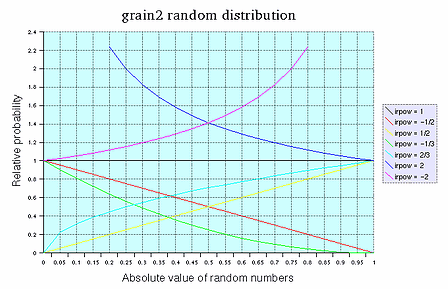
\includegraphics[scale=1]{grain2_rand-448x289} 


 A graph of distributions for different values of irpow.


 \emph{iseed}
 (optional, default=0) -- seed value for random number generator (positive integer in the range 1 to 2147483646 (2 \^{} 31 - 2)). Zero or negative value seeds from current time (this is also the default). 


 \emph{imode}
 (optional, default=0) -- sum of the following values: 


 
\begin{itemize}
\item 

 \emph{64:}
 synchronize start phase of grains to kcps.

\item 

 \emph{32:}
 start all grains at integer sample location. This may be faster in some cases, however it also makes the timing of grain envelopes less accurate.

\item 

 \emph{16:}
 do not render grains with start time less than zero. (see the image below; this option turns off grains marked with red on the image).

\item 

 \emph{8:}
 interpolate window waveform (slower).

\item 

 \emph{4:}
 do not interpolate grain waveform (fast, but lower quality).

\item 

 \emph{2:}
 grain frequency is continuously modified by \emph{kcps}
 and \emph{kfmd}
 (by default, each grain keeps the frequency it was launched with). This may be slower at high control rates. It also controls phase modulation (kphs).

\item 

 \emph{1:}
 skip initialization.


\end{itemize}


 


 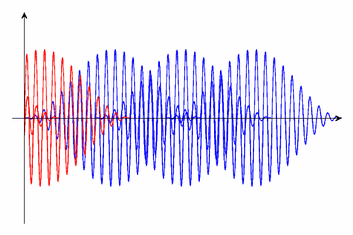
\includegraphics[scale=1]{grain3_2} 


 A diagram showing grains with a start time less than zero in red.
\subsection*{Performance}


 \emph{ar}
 -- output signal. 


 \emph{kcps}
 -- grain frequency in Hz. 


 \emph{kphs}
 -- grain phase. This is the location in the grain waveform table, expressed as a fraction (between 0 to 1) of the table length. 


 \emph{kfmd}
 -- random variation (bipolar) in grain frequency in Hz. 


 \emph{kpmd}
 -- random variation (bipolar) in start phase. 


 \emph{kgdur}
 -- grain duration in seconds. \emph{kgdur}
 also controls the duration of already active grains (actually the speed at which the window function is read). This behavior does not depend on the \emph{imode}
 flags. 


 \emph{kdens}
 -- number of grains per second. 


 \emph{kfrpow}
 -- distribution of random frequency variation (see irpow). 


 \emph{kprpow}
 -- distribution of random phase variation (see irpow). Setting kphs and kpmd to 0.5, and kprpow to 0 will emulate \emph{grain2}
. 


 \emph{kfn}
 -- function table containing grain waveform. Table number can be changed at k-rate (this is useful to select from a set of band-limited tables generated by GEN30, to avoid aliasing). 


 


\begin{tabular}{cc}
\textbf{Note}
 \\
� &

 \emph{grain3}
 internally uses the same random number generator as \emph{rnd31}
. So reading \emph{its documentation}
 is also recommended. 


\end{tabular}

\subsection*{Examples}


  Here is an example of the grain3 opcode. It uses the files \emph{grain3.orc}
 and \emph{grain3.sco}
. 


 \textbf{Example 1. Example of the grain3 opcode.}

\begin{lstlisting}
/* grain3.orc */
sr	=  48000
kr	=  1000
ksmps   =  48
nchnls	=  1

/* Bartlett window */
itmp	ftgen 1, 0, 16384, 20, 3, 1
/* sawtooth wave */
itmp	ftgen 2, 0, 16384, 7, 1, 16384, -1
/* sine */
itmp	ftgen 4, 0, 1024, 10, 1
/* window for "soft sync" with 1/32 overlap */
itmp	ftgen 5, 0, 16384, 7, 0, 256, 1, 7936, 1, 256, 0, 7936, 0
/* generate bandlimited sawtooth waves */
itmp	ftgen 3, 0, 4096, -30, 2, 1, 2048
icnt	=  0
loop01:
; 100 tables for 8 octaves from 30 Hz
ifrq	=  30 * exp(log(2) * 8 * icnt / 100)
itmp	ftgen icnt + 100, 0, 4096, -30, 3, 1, sr / (2 * ifrq)
icnt	=  icnt + 1
	if (icnt < 99.5) igoto loop01
/* convert frequency to table number */
#define FRQ2FNUM(xout'xcps'xbsfn) #

$xout	=  int(($xbsfn) + 0.5 + (100 / 8) * log(($xcps) / 30) / log(2))
$xout	limit $xout, $xbsfn, $xbsfn + 99

#

/* instr 1: pulse width modulated grains */

	instr 1

kfrq	=  523.25		; frequency
$FRQ2FNUM(kfnum'kfrq'100)	; table number
kfmd	=  kfrq * 0.02		; random variation in frequency
kgdur	=  0.2			; grain duration
kdens	=  200			; density
iseed	=  1			; random seed

kphs	oscili 0.45, 1, 4	; phase

a1	grain3	kfrq, 0, kfmd, 0.5, kgdur, kdens, 100,		\
		kfnum, 1, -0.5, 0, iseed, 2
a2	grain3	kfrq, 0.5 + kphs, kfmd, 0.5, kgdur, kdens, 100,	\
		kfnum, 1, -0.5, 0, iseed, 2

; de-click
aenv	linseg 0, 0.01, 1, p3 - 0.05, 1, 0.04, 0, 1, 0

	out aenv * 2250 * (a1 - a2)

	endin

/* instr 2: phase variation */

	instr 2

kfrq	=  220			; frequency
$FRQ2FNUM(kfnum'kfrq'100)	; table number
kgdur	=  0.2			; grain duration
kdens	=  200			; density
iseed	=  2			; random seed

kprdst	expon 0.5, p3, 0.02	; distribution

a1	grain3	kfrq, 0.5, 0, 0.5, kgdur, kdens, 100,		\
		kfnum, 1, 0, -kprdst, iseed, 64

; de-click
aenv	linseg 0, 0.01, 1, p3 - 0.05, 1, 0.04, 0, 1, 0

	out aenv * 1500 * a1

	endin

/* instr 3: "soft sync" */

	instr 3

kdens	=  130.8		; base frequency
kgdur	=  2 / kdens		; grain duration

kfrq	expon 880, p3, 220	; oscillator frequency
$FRQ2FNUM(kfnum'kfrq'100)	; table number

a1	grain3 kfrq, 0, 0, 0, kgdur, kdens, 3, kfnum, 5, 0, 0, 0, 2
a2	grain3 kfrq, 0.667, 0, 0, kgdur, kdens, 3, kfnum, 5, 0, 0, 0, 2

; de-click
aenv	linseg 0, 0.01, 1, p3 - 0.05, 1, 0.04, 0, 1, 0

	out aenv * 10000 * (a1 - a2)

	endin
/* grain3.orc */
        
\end{lstlisting}
\begin{lstlisting}
/* grain3.sco */
t 0 60
i 1 0 3
i 2 4 3
i 3 8 3
e
/* grain3.sco */
        
\end{lstlisting}
\subsection*{See Also}


 \emph{grain2}

\subsection*{Credits}


 


 


\begin{tabular}{c}
Author: Istvan Varga

\end{tabular}



 


 New in version 4.15


 Updated April 2002 by Istvan Varga
%\hline 


\begin{comment}
\begin{tabular}{lcr}
Previous &Home &Next \\
grain2 &Up &granule

\end{tabular}


\end{document}
\end{comment}
